\section{实验}
\frame
{
	\frametitle{\secname~ }
	\begin{block}{环境配置}
		搭建的训练环境、实现的一些细节
	\end{block}
	\begin{block}{实验结果}
		实验结果和分析
	\end{block}
}

\subsection*{环境配置}
\frame{
	\frametitle{训练环境}
	\vspace{-1em}
	\begin{block}{}
		\small
		本文利用 Bsuite 强化学习工具套件,实现了一篇文献\footnote{Oh \& Junhyuk, Discovering {{Reinforcement Learning Algorithms}}, NeurIPS 2020}中设计的表格型网格世界环境。
	\end{block}
	\begin{figure}[h!]
		\centering
		\includegraphics[height=0.4\textheight ]{image/chap04/simple_grid_world.pdf}
		\caption{网格世界}
		\label{fig:simple-gridworld}
	\end{figure}
	
}
\frame{
	\frametitle{实现细节}
	\begin{block}{}
		\begin{itemize}
			\item 使用20维预测向量$y \in \mathcal{R}^{20}$
			\item 每20步更新一次
			\item LSTM使用两层的MLP
			\item 使用 pytorch 和 Bsuite 实现算法
		\end{itemize}
	\end{block}
}

\subsection*{实验结果}
\frame{
	\frametitle{实验结果}
	\begin{figure}[h!]
		\centering
		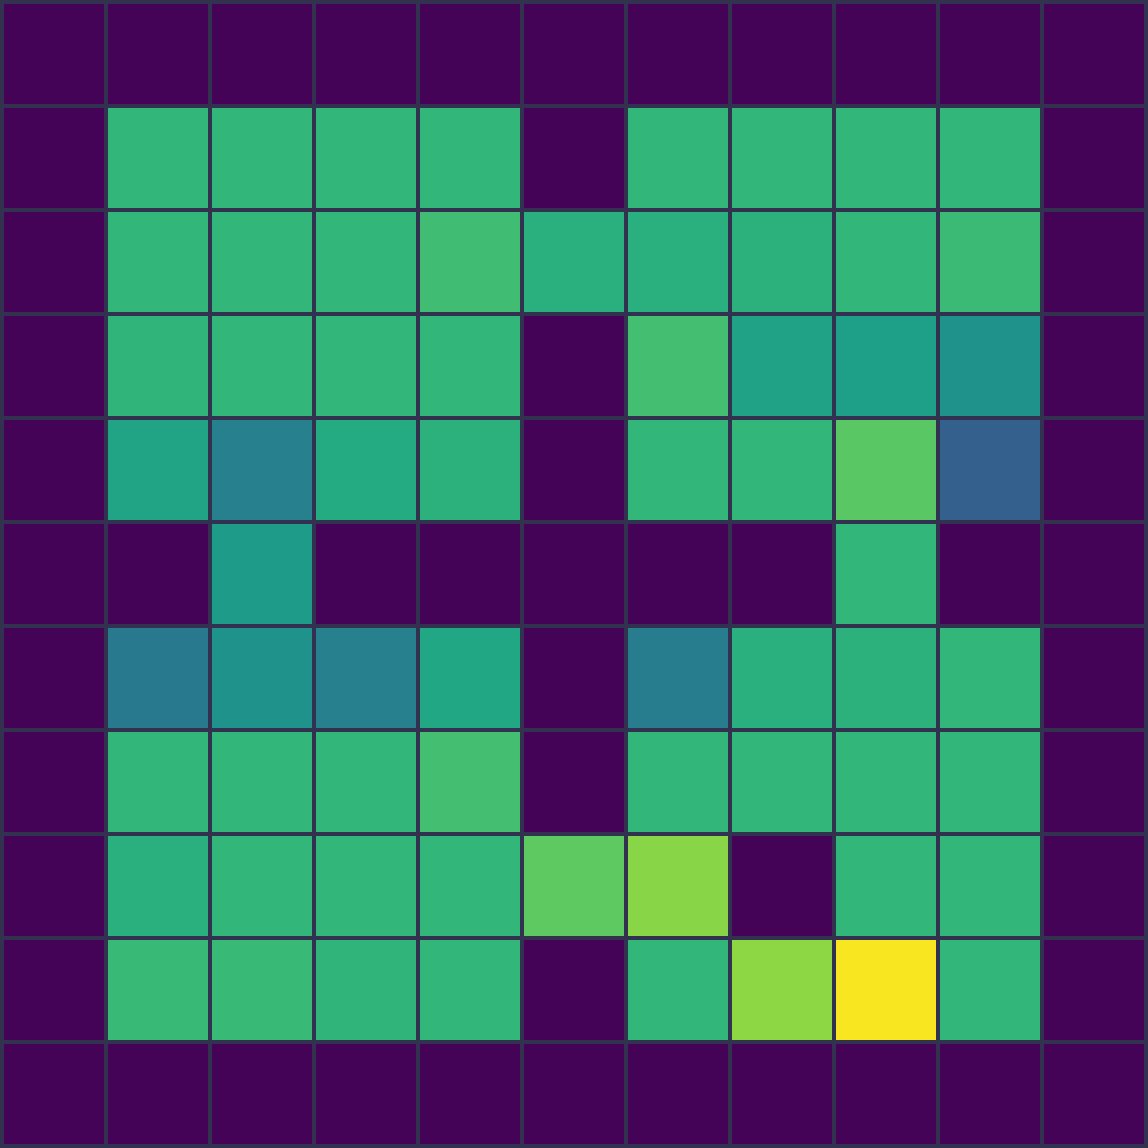
\includegraphics[width=0.09\textwidth]{image/chap04/prediction/0.png}
		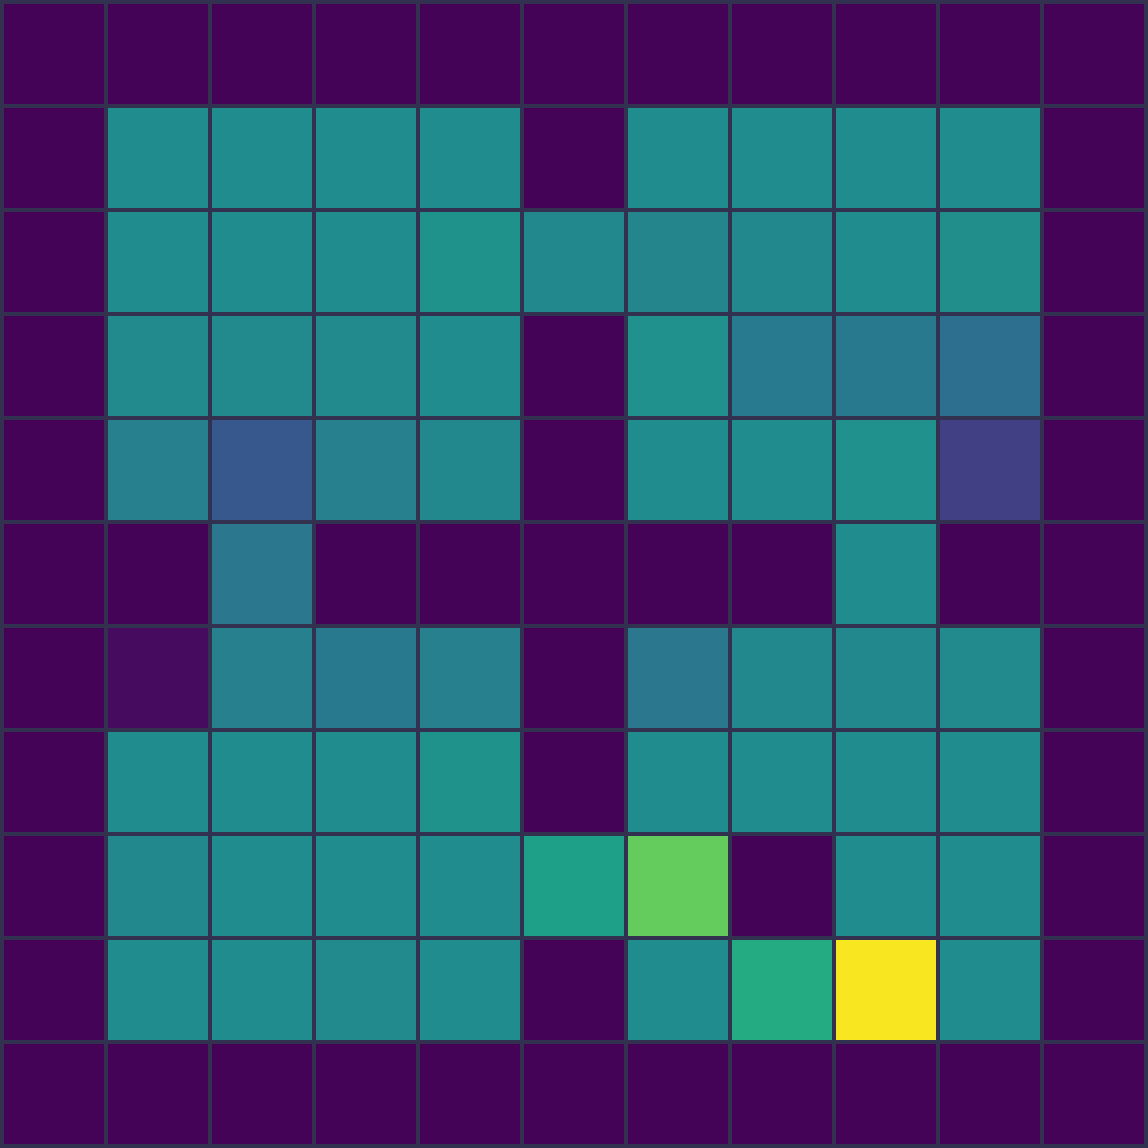
\includegraphics[width=0.09\textwidth]{image/chap04/prediction/1.png}
		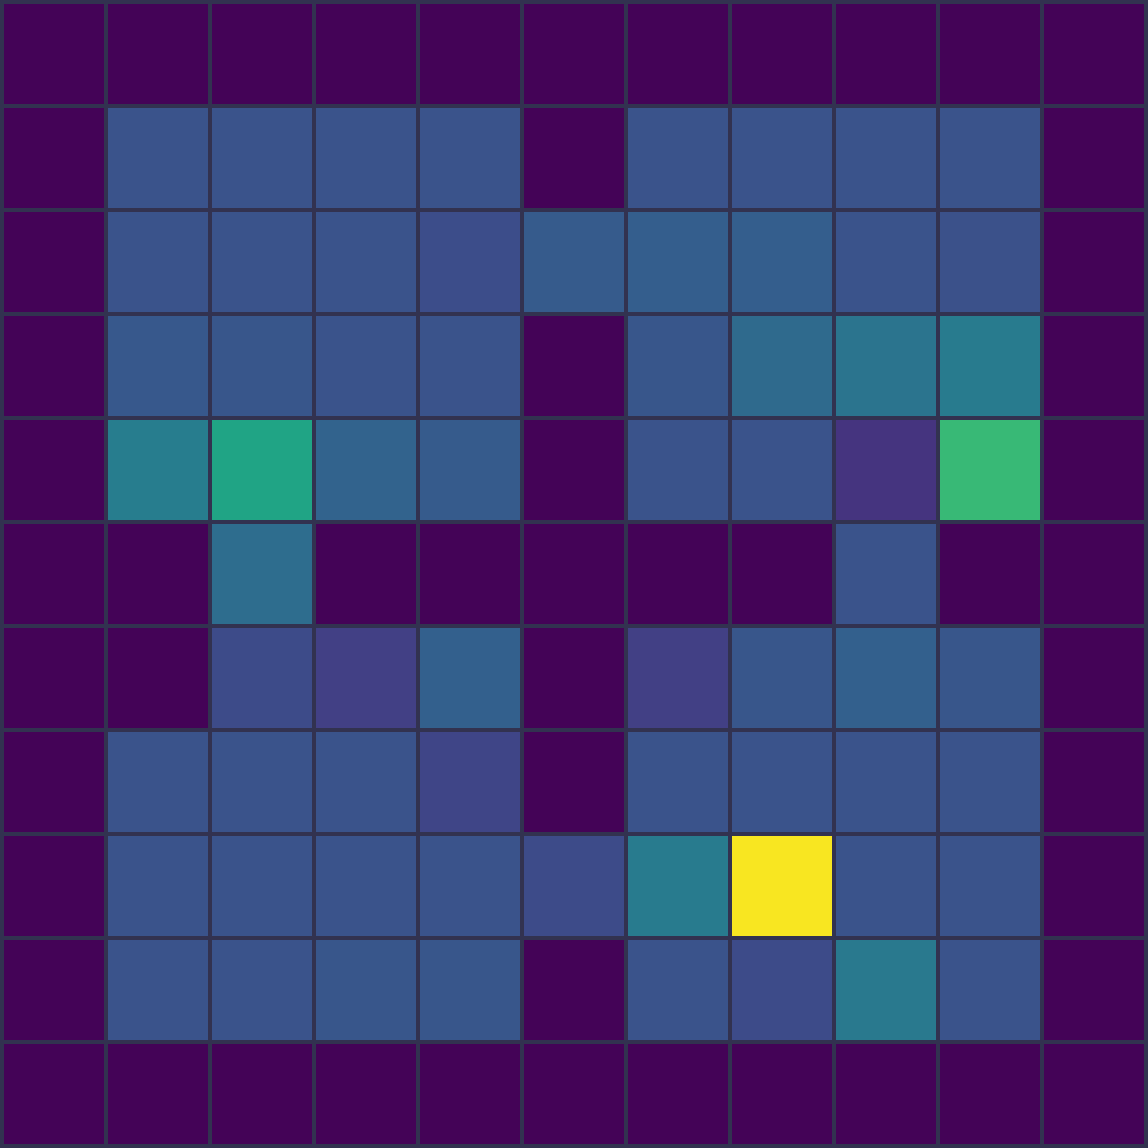
\includegraphics[width=0.09\textwidth]{image/chap04/prediction/2.png}
		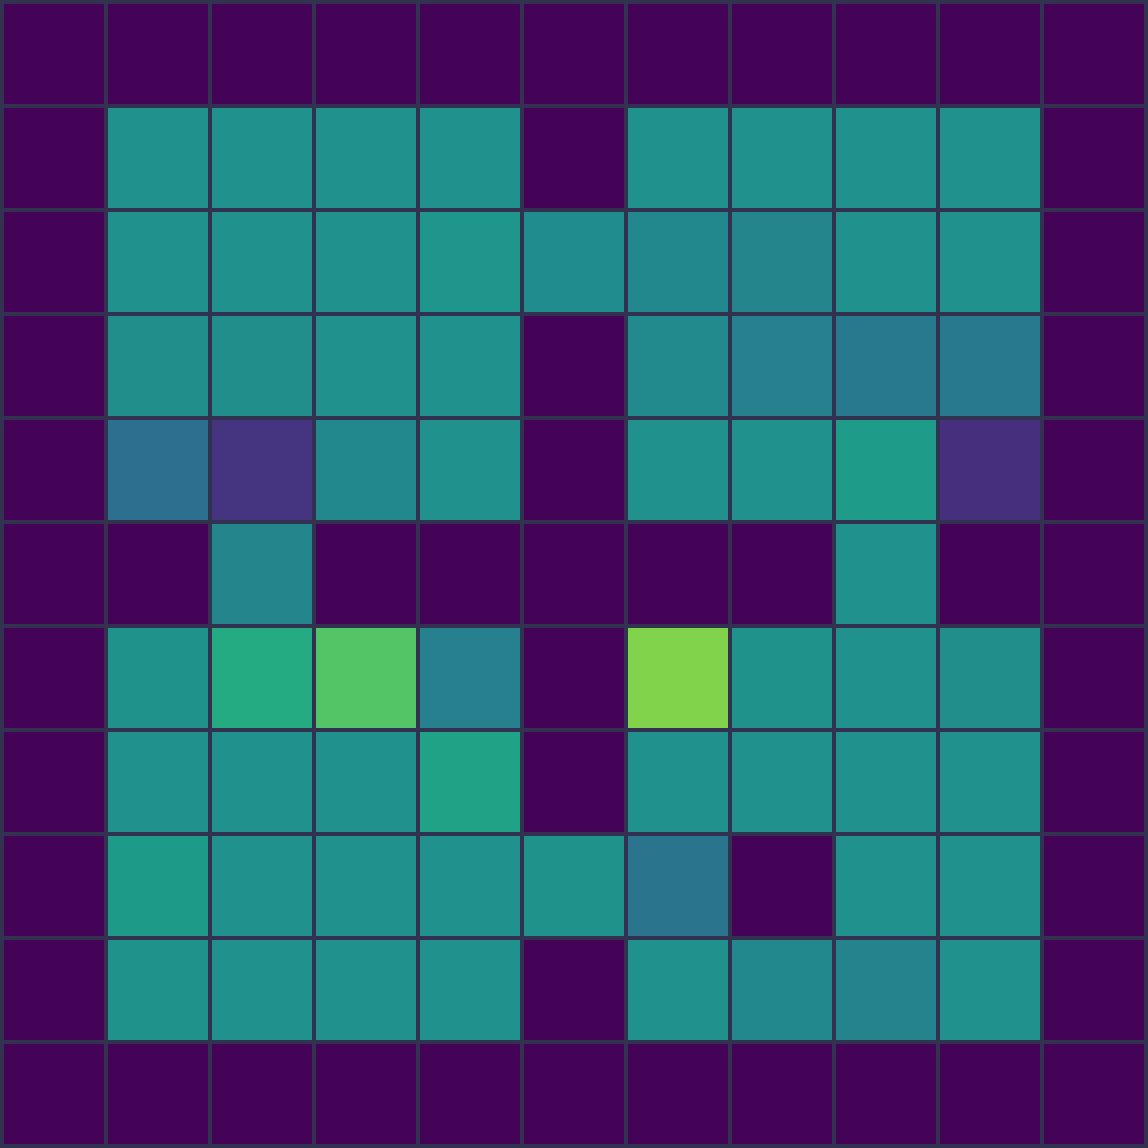
\includegraphics[width=0.09\textwidth]{image/chap04/prediction/3.png}
		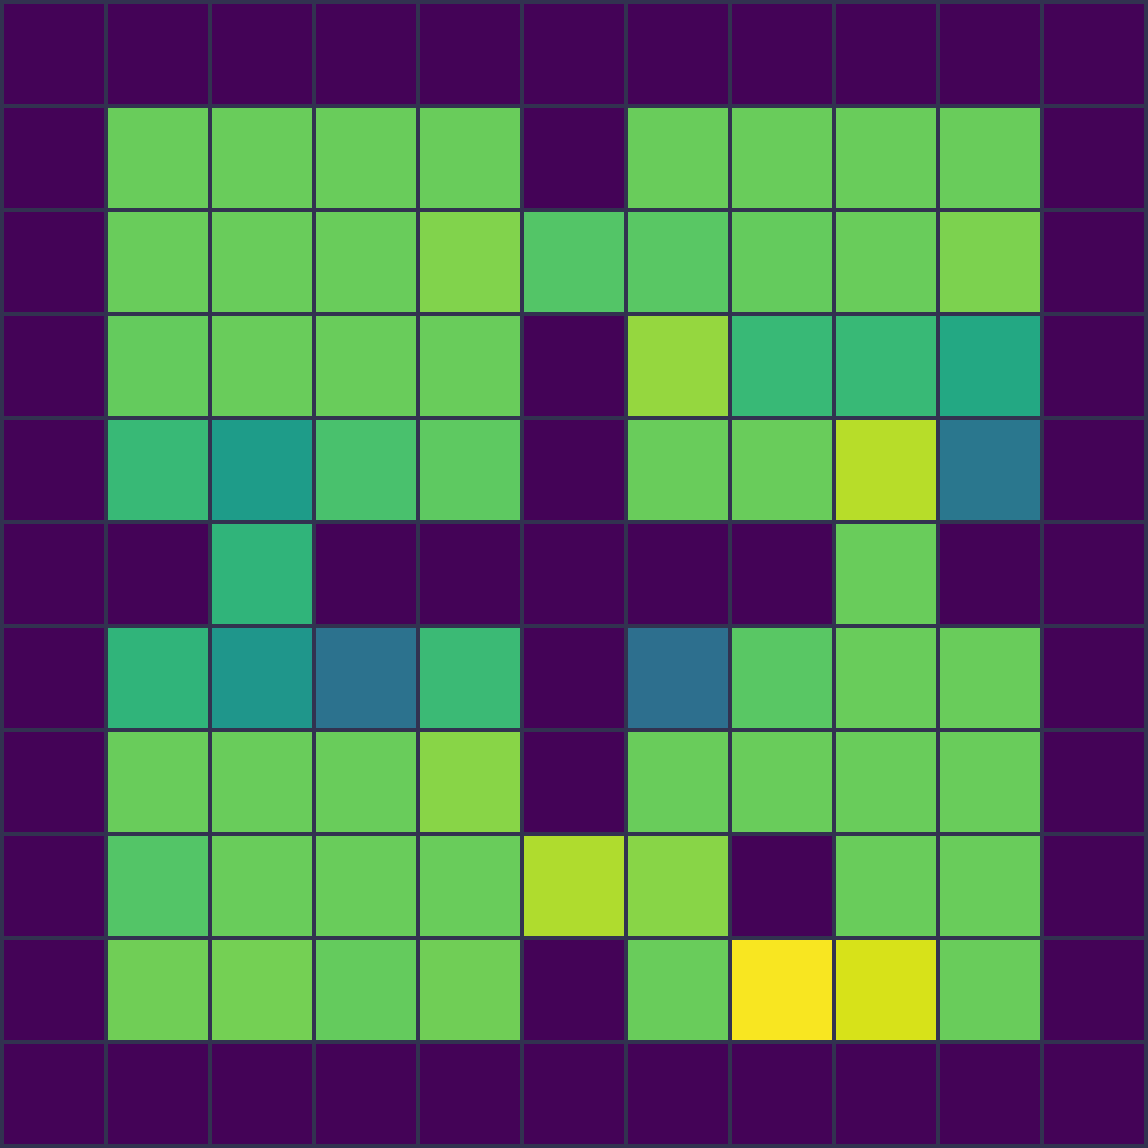
\includegraphics[width=0.09\textwidth]{image/chap04/prediction/4.png}
		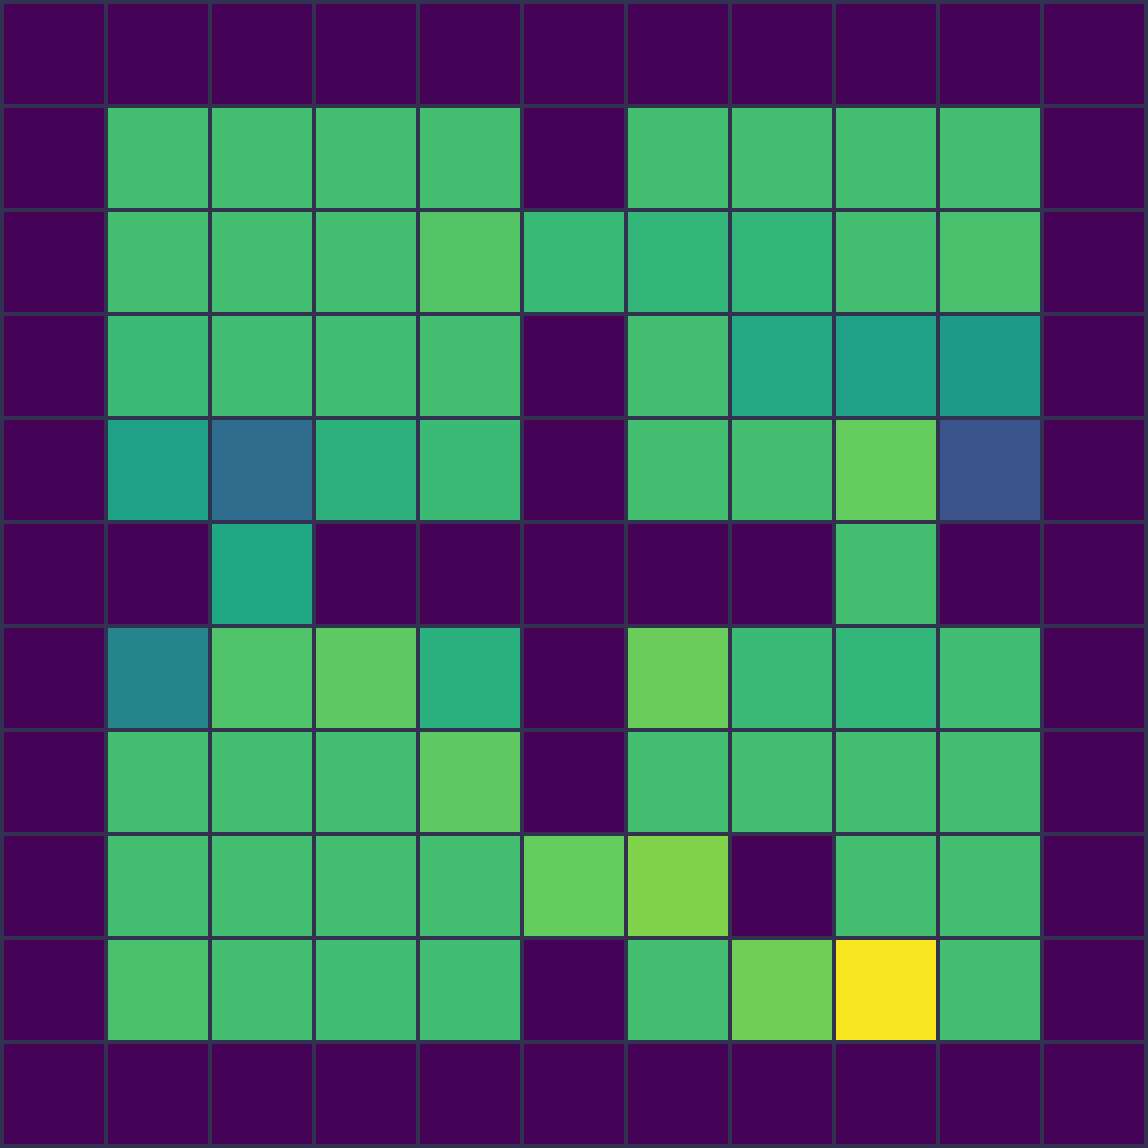
\includegraphics[width=0.09\textwidth]{image/chap04/prediction/5.png}
		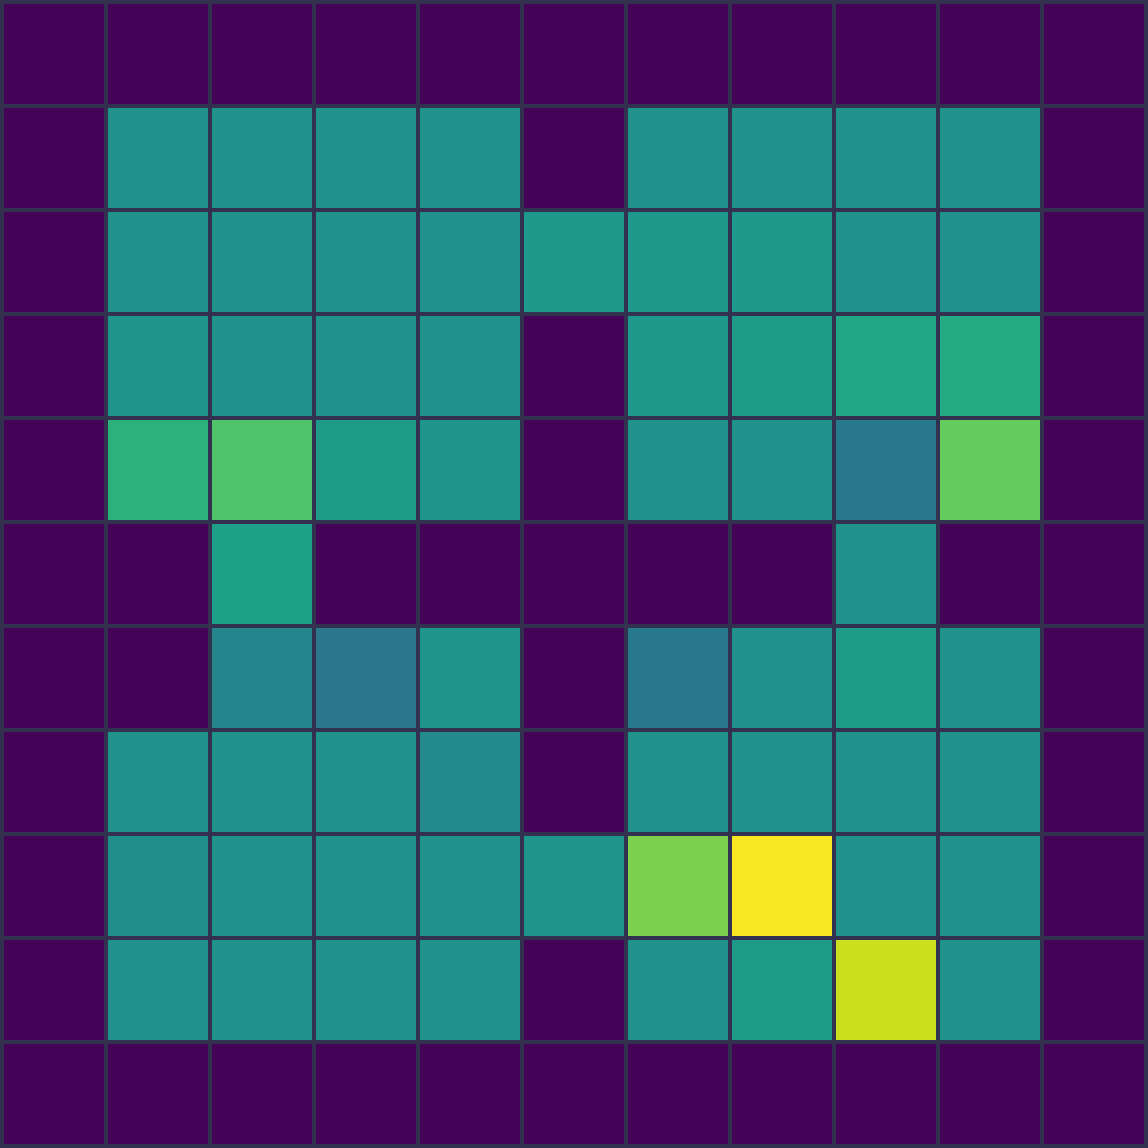
\includegraphics[width=0.09\textwidth]{image/chap04/prediction/6.png}
		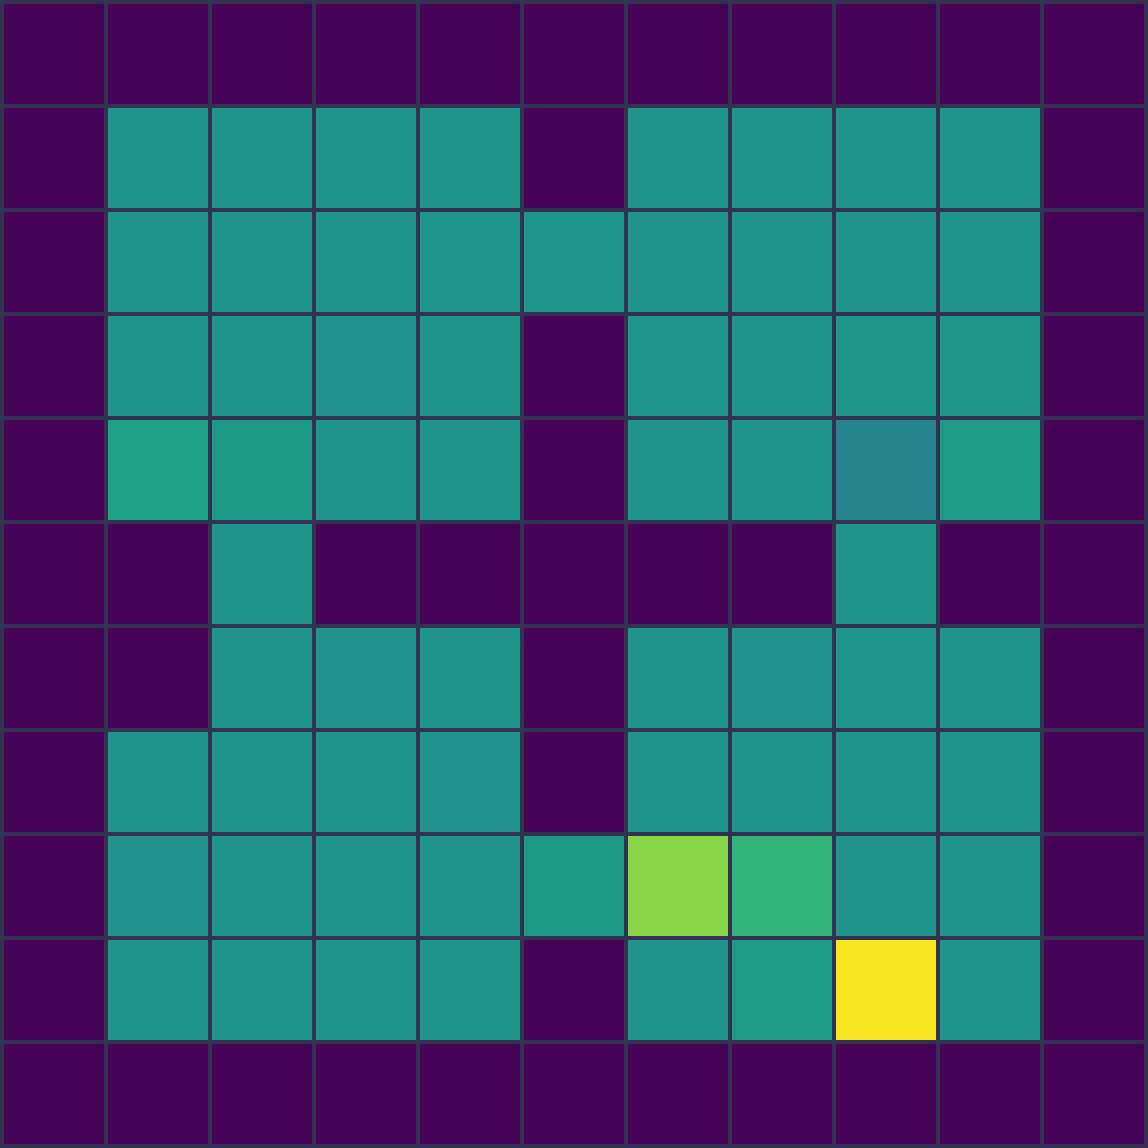
\includegraphics[width=0.09\textwidth]{image/chap04/prediction/7.png}
		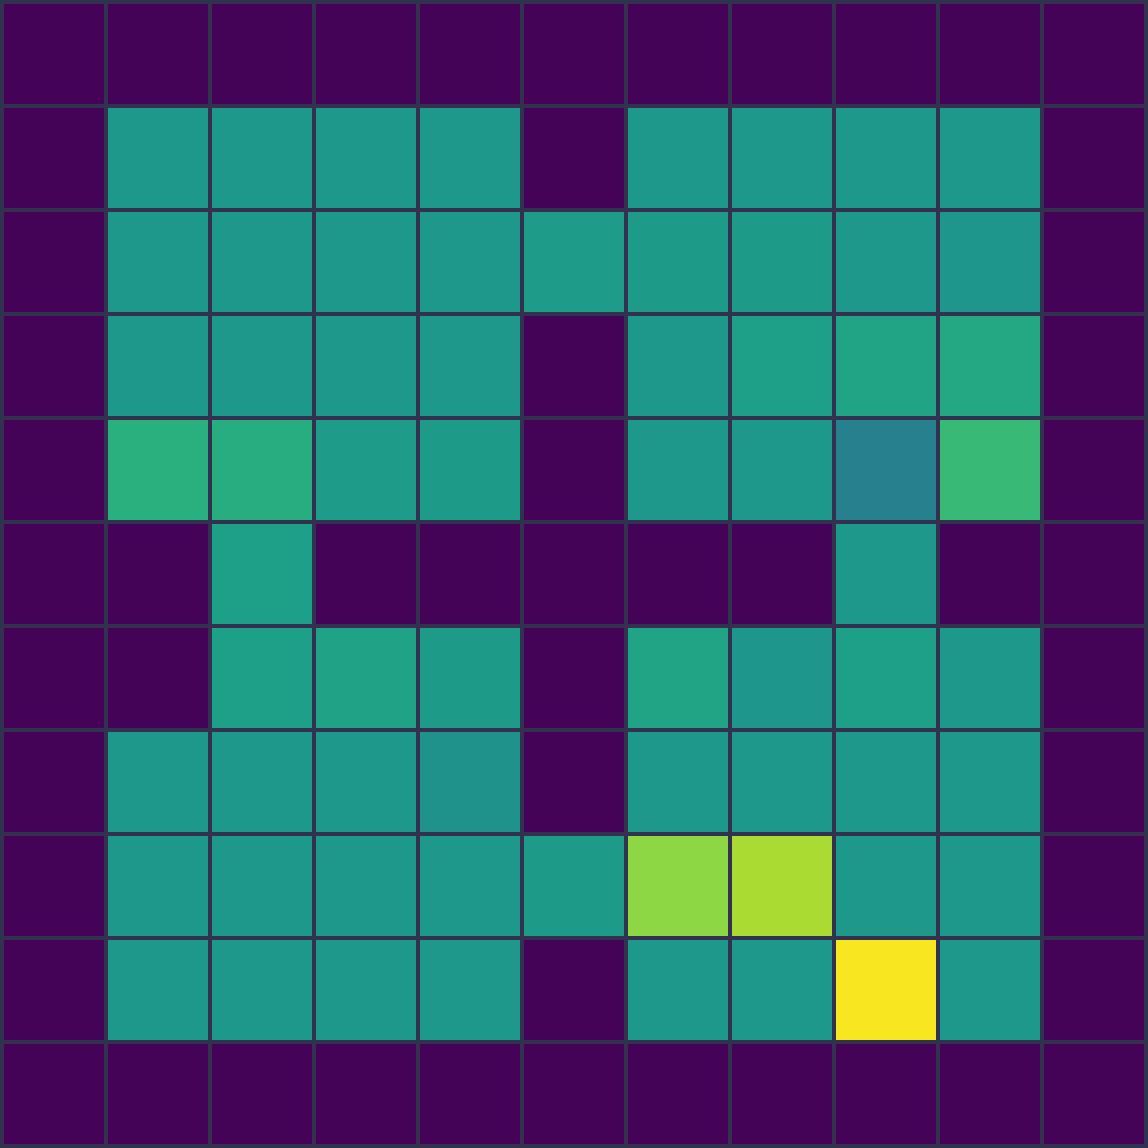
\includegraphics[width=0.09\textwidth]{image/chap04/prediction/8.png}
		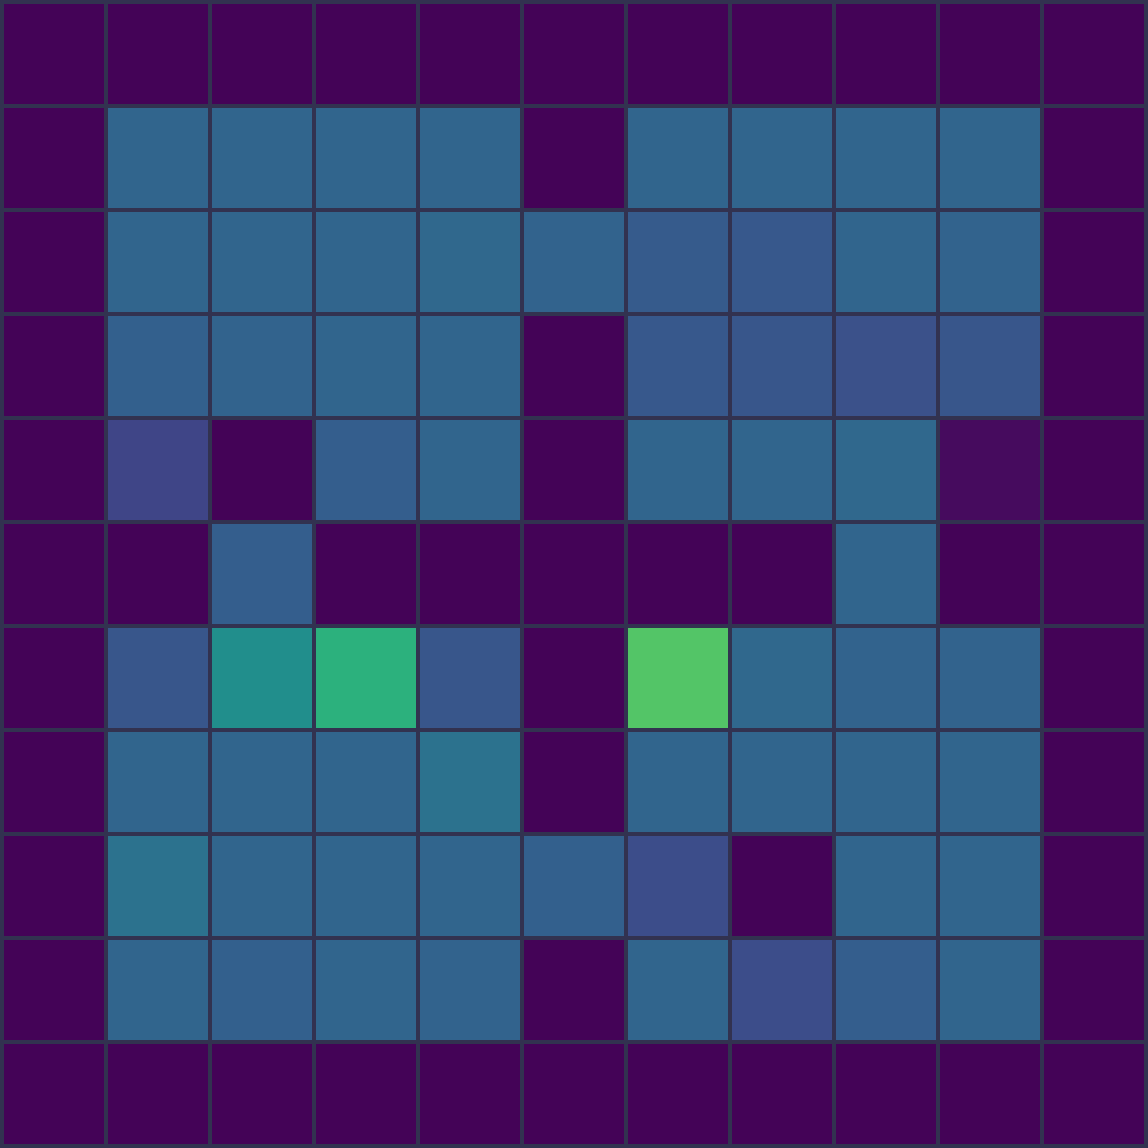
\includegraphics[width=0.09\textwidth]{image/chap04/prediction/9.png}
		\\
		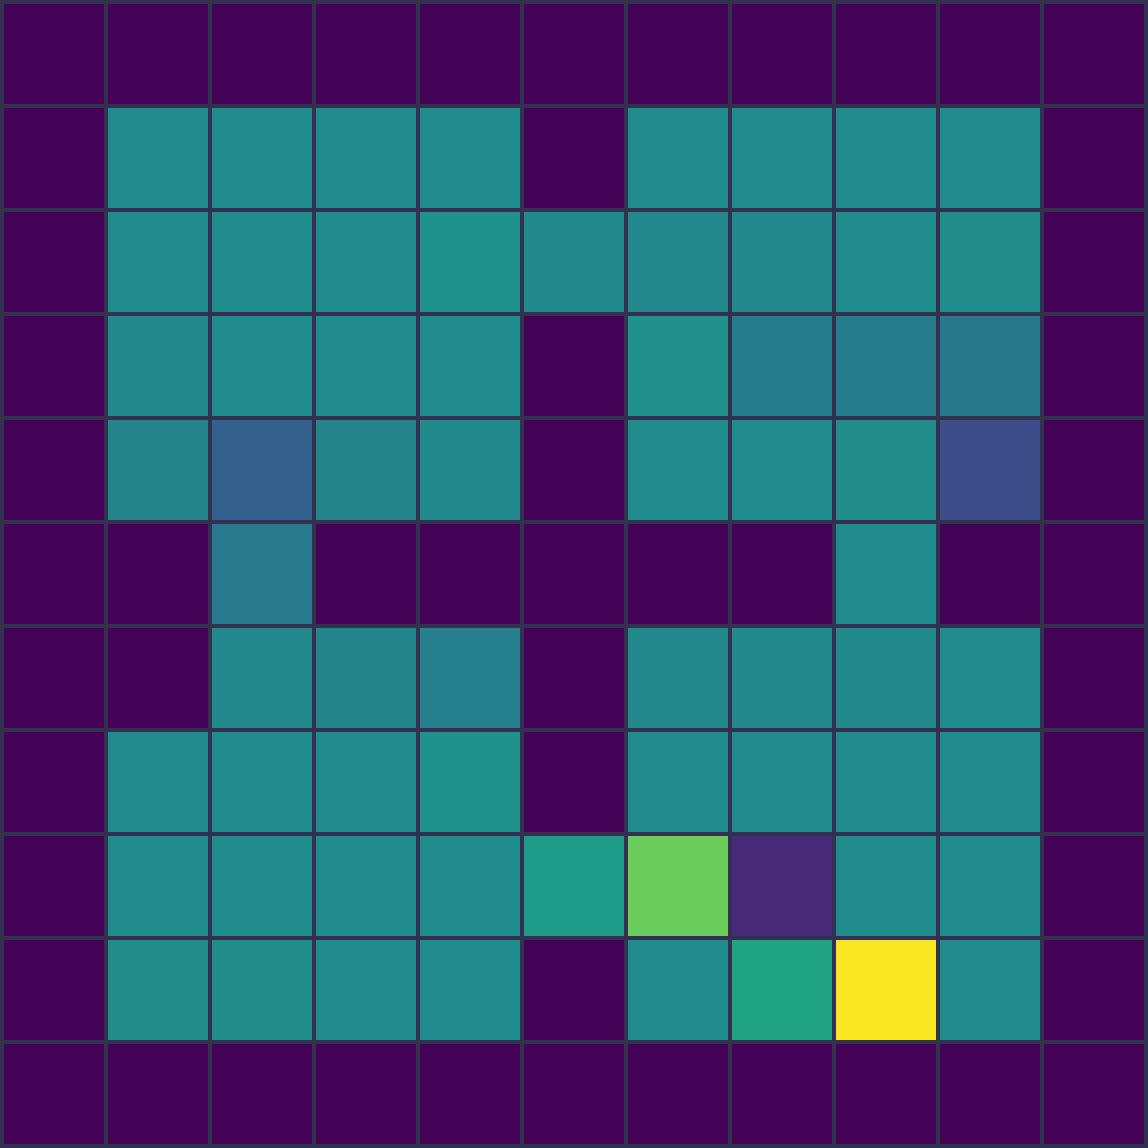
\includegraphics[width=0.09\textwidth]{image/chap04/prediction/10.png}
		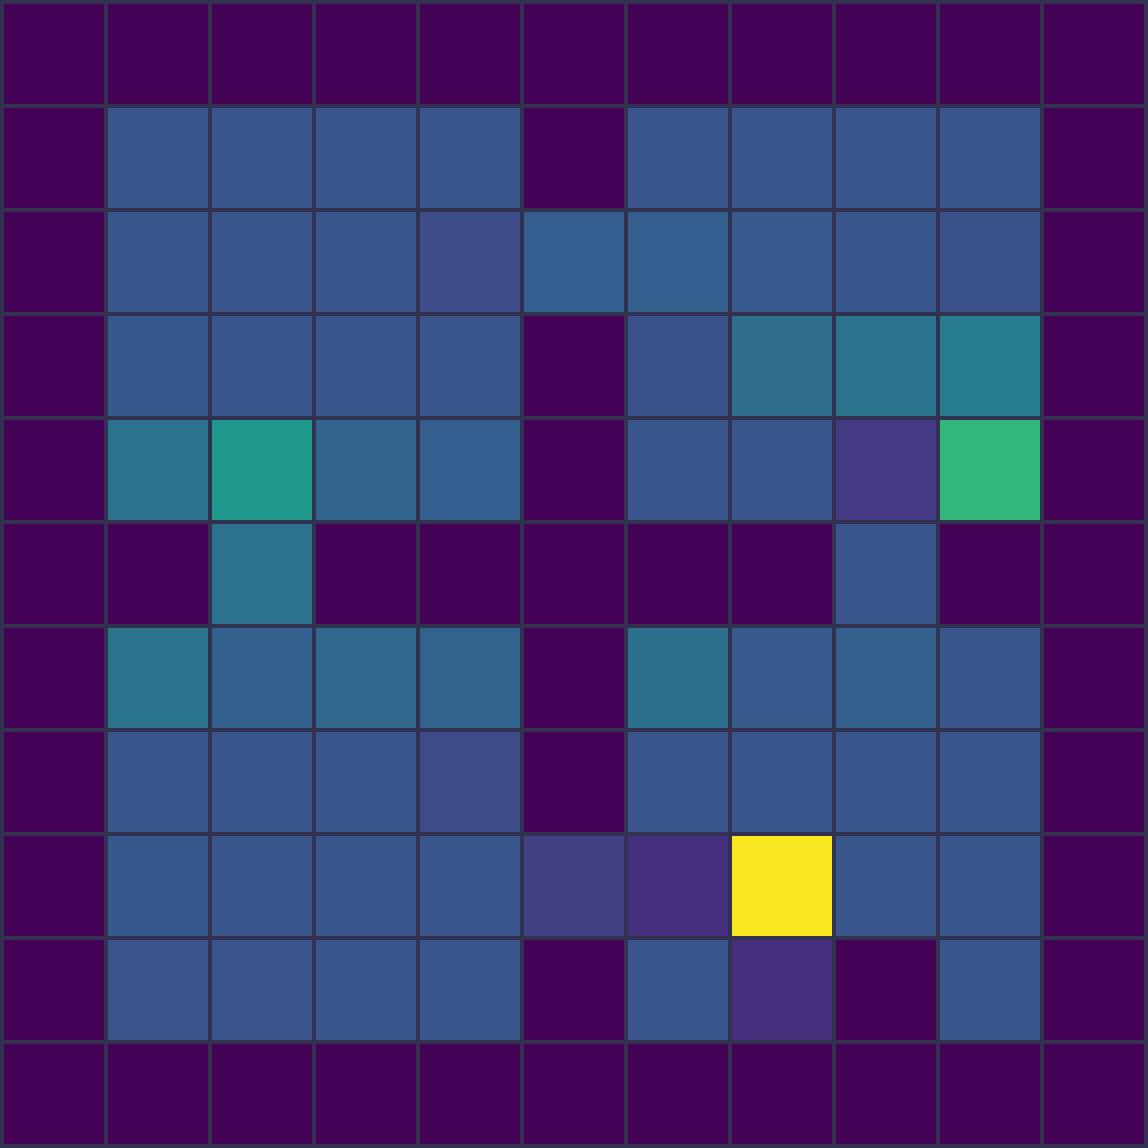
\includegraphics[width=0.09\textwidth]{image/chap04/prediction/11.png}
		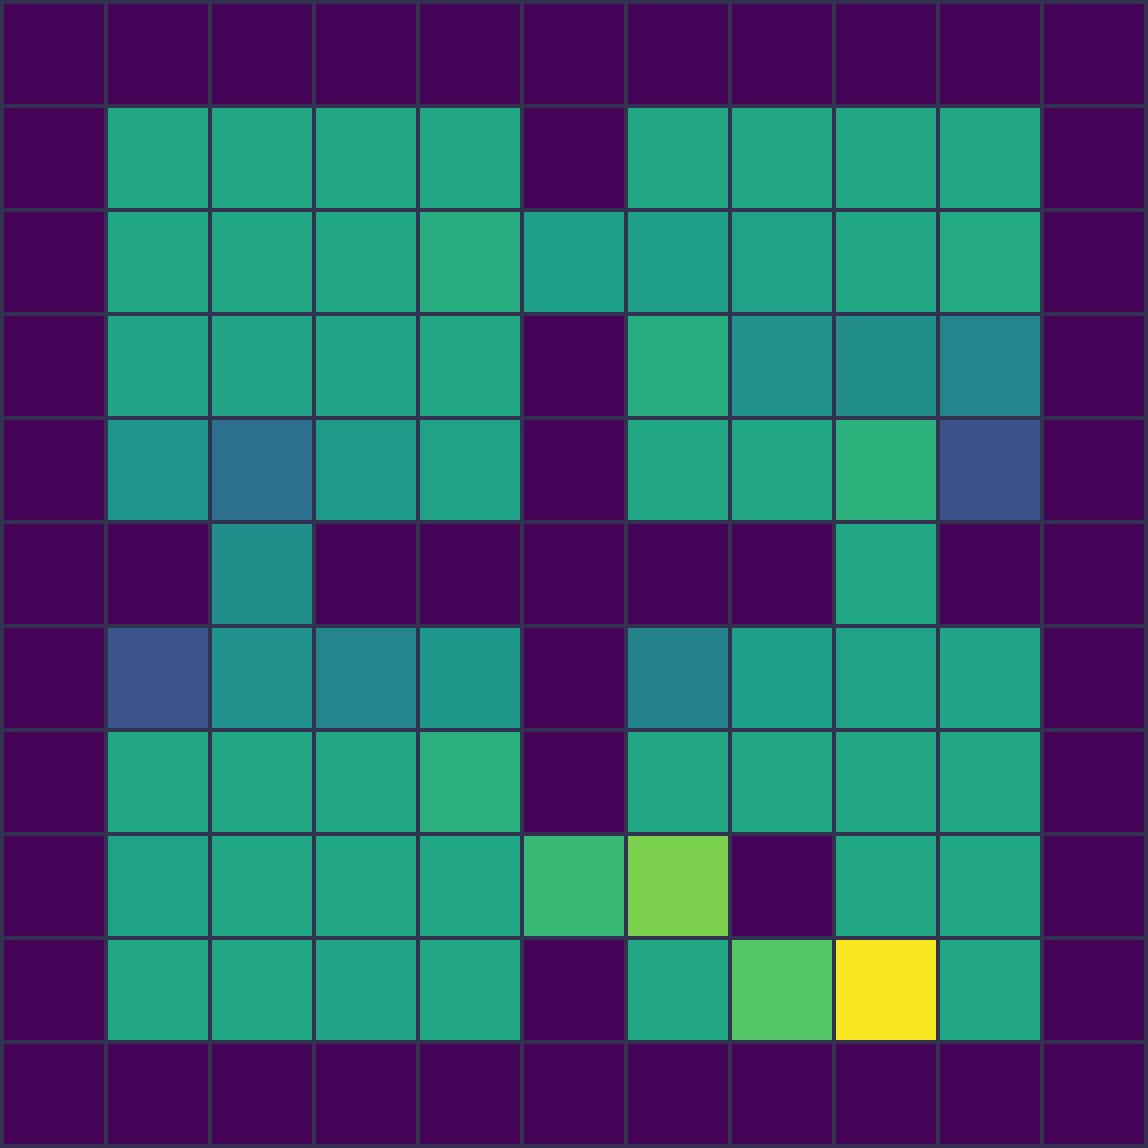
\includegraphics[width=0.09\textwidth]{image/chap04/prediction/12.png}
		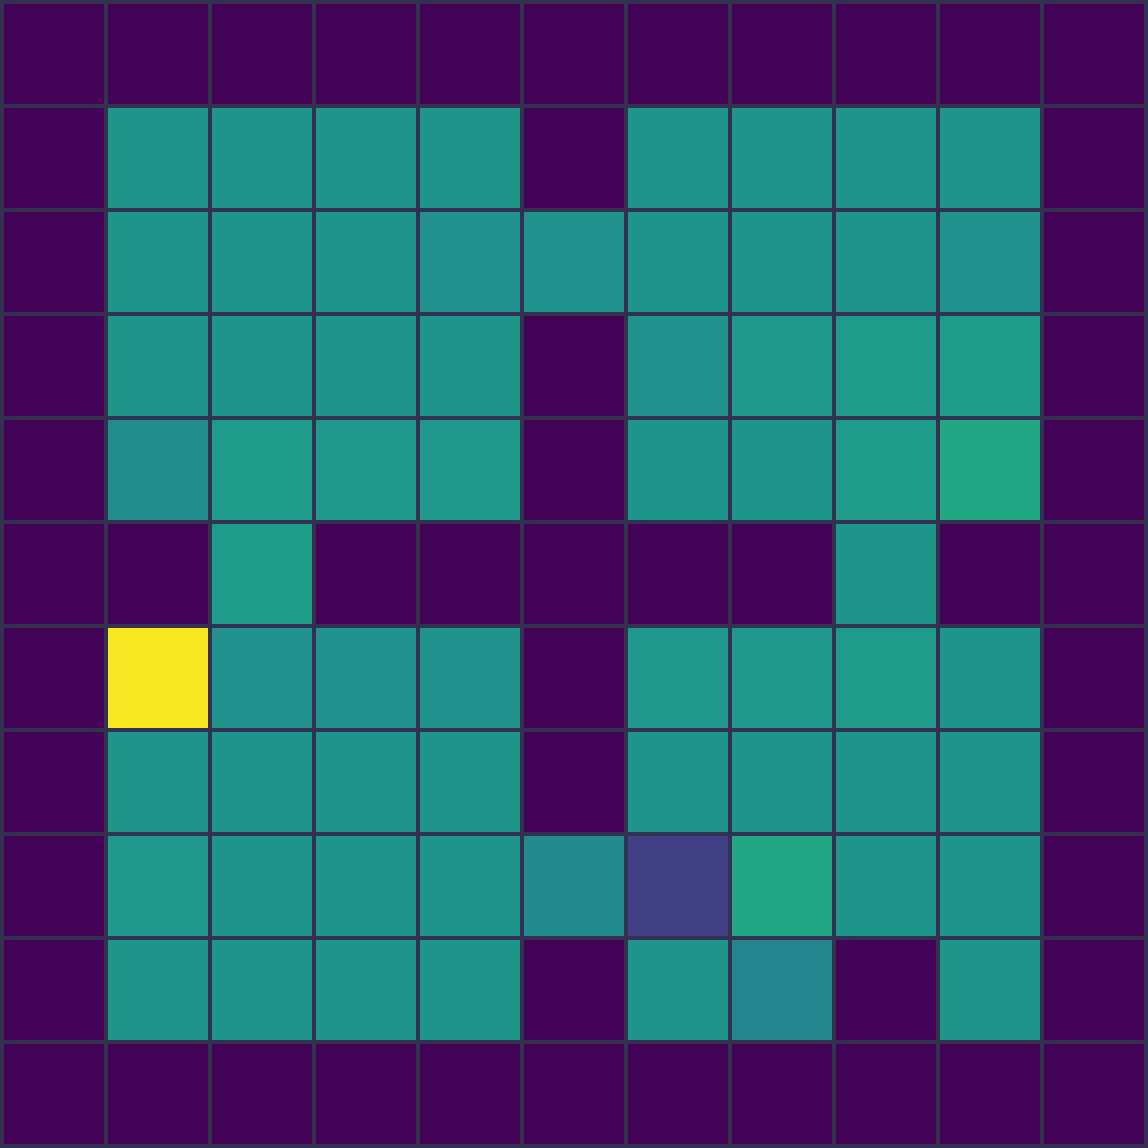
\includegraphics[width=0.09\textwidth]{image/chap04/prediction/13.png}
		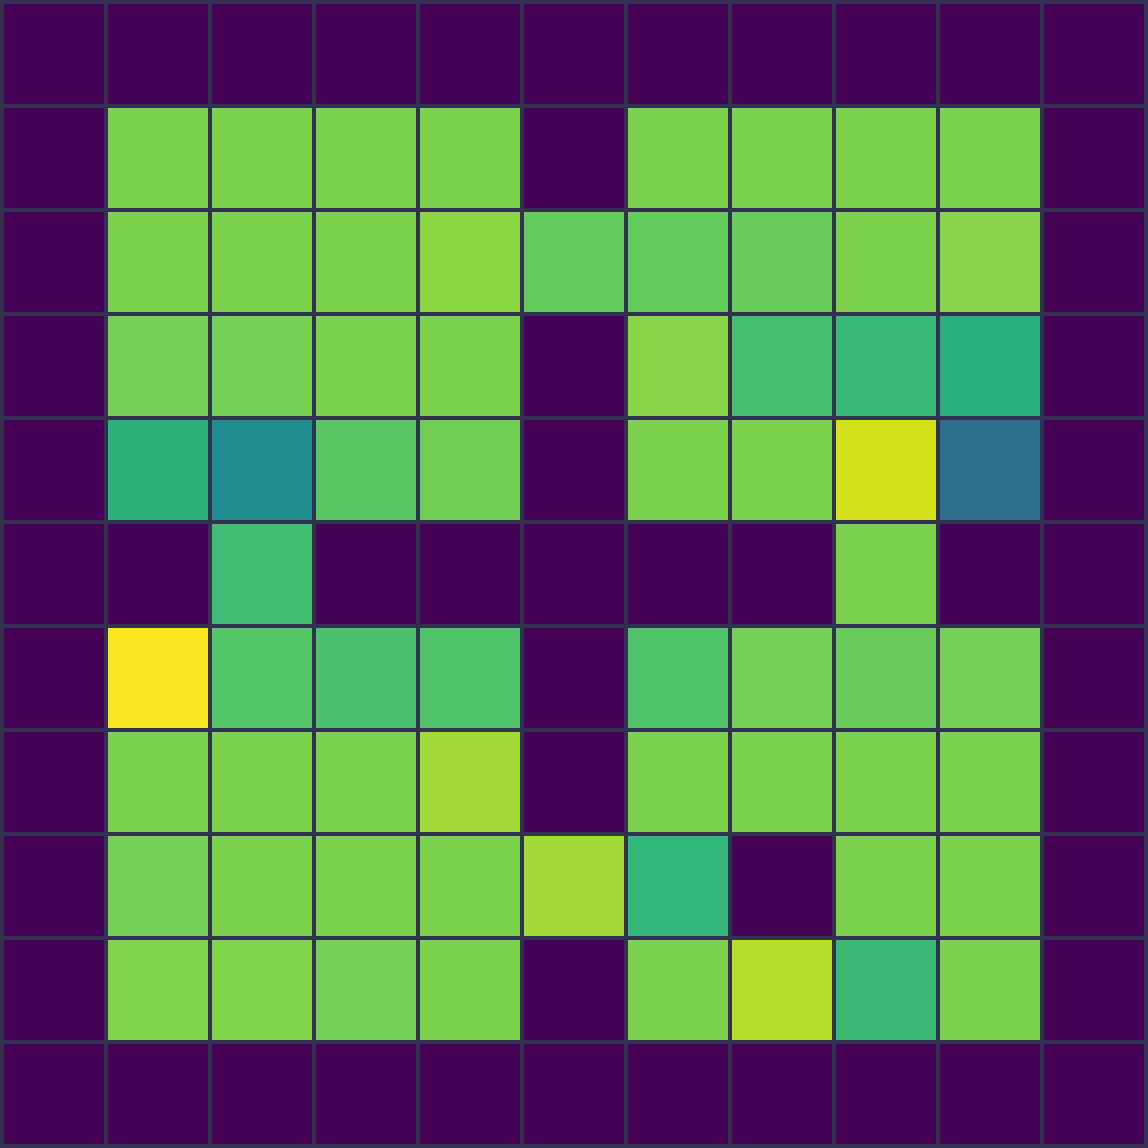
\includegraphics[width=0.09\textwidth]{image/chap04/prediction/14.png}
		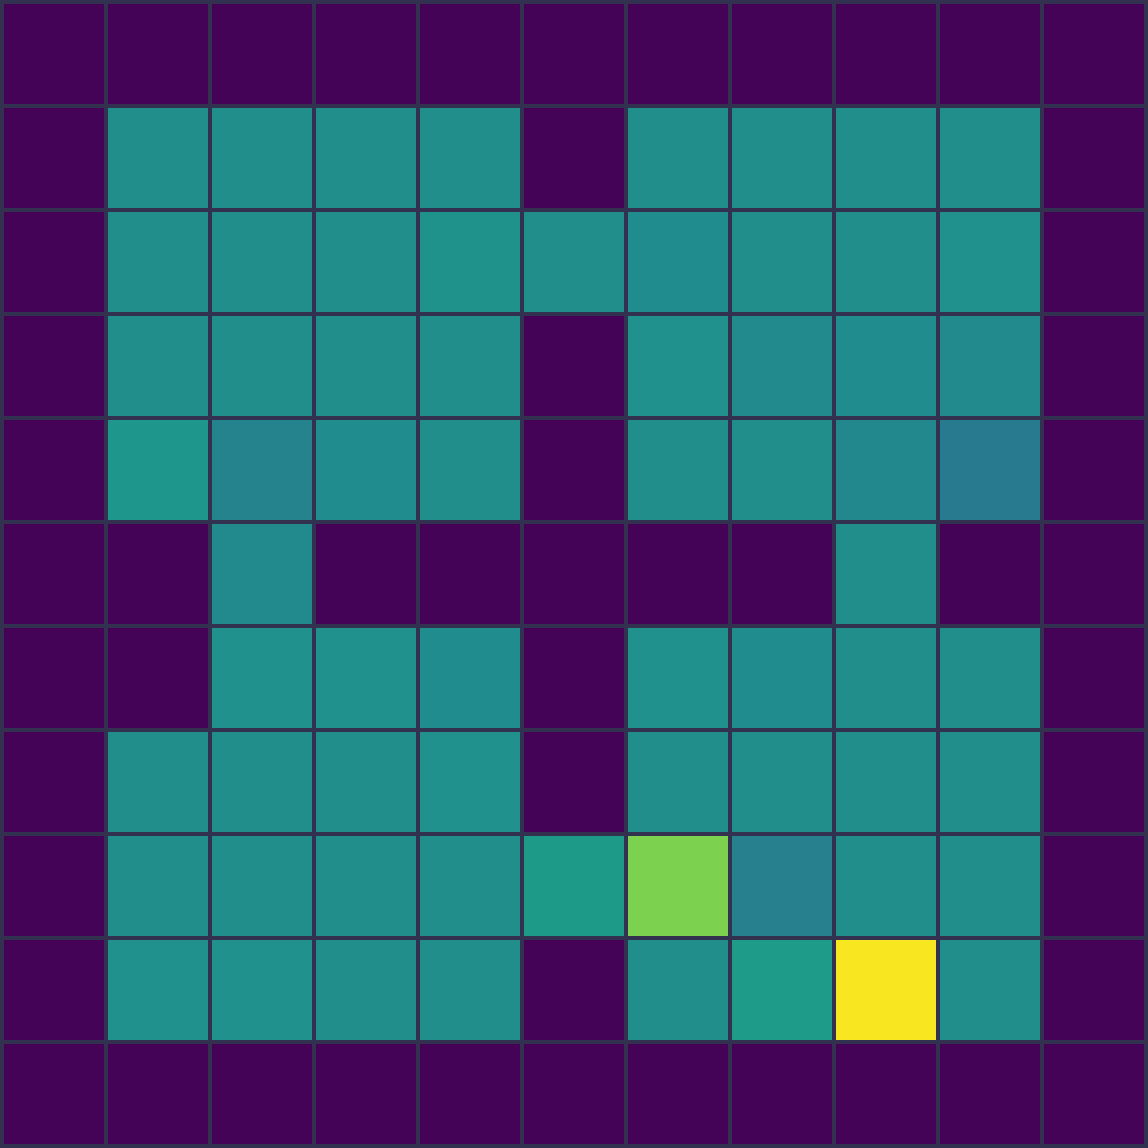
\includegraphics[width=0.09\textwidth]{image/chap04/prediction/15.png}
		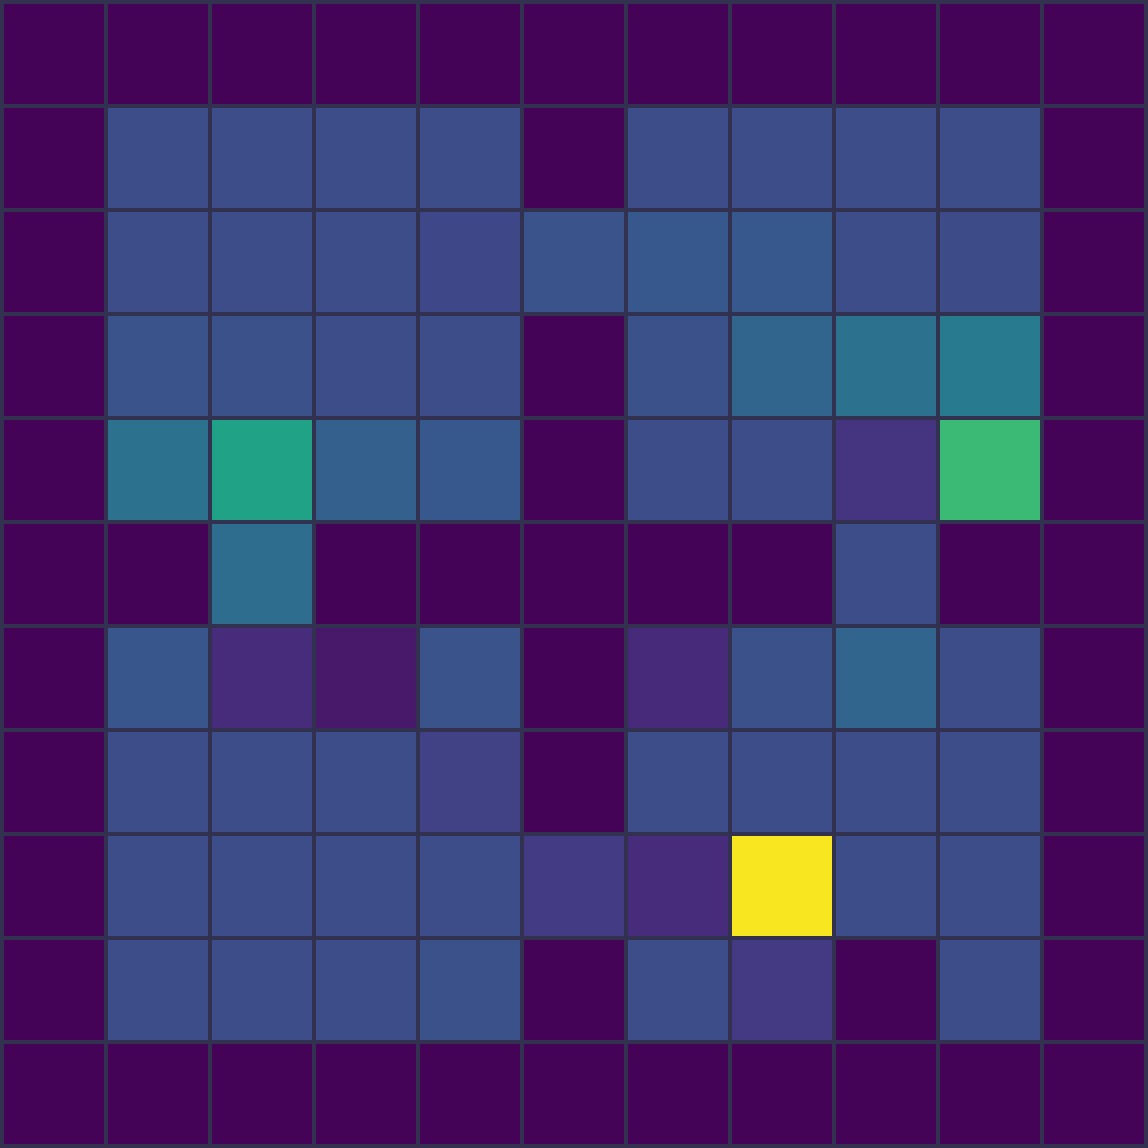
\includegraphics[width=0.09\textwidth]{image/chap04/prediction/16.png}
		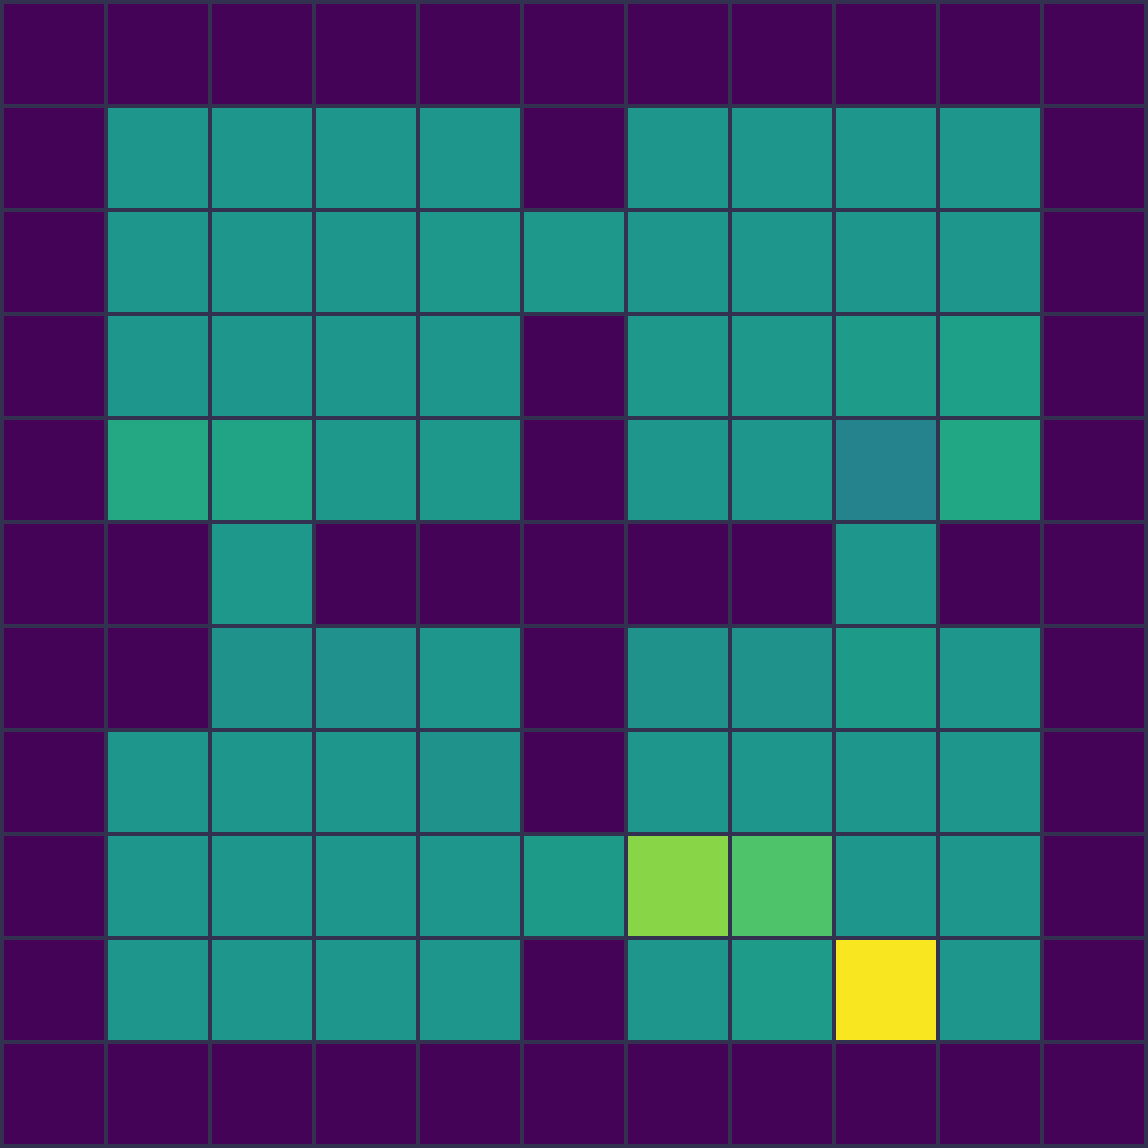
\includegraphics[width=0.09\textwidth]{image/chap04/prediction/17.png}
		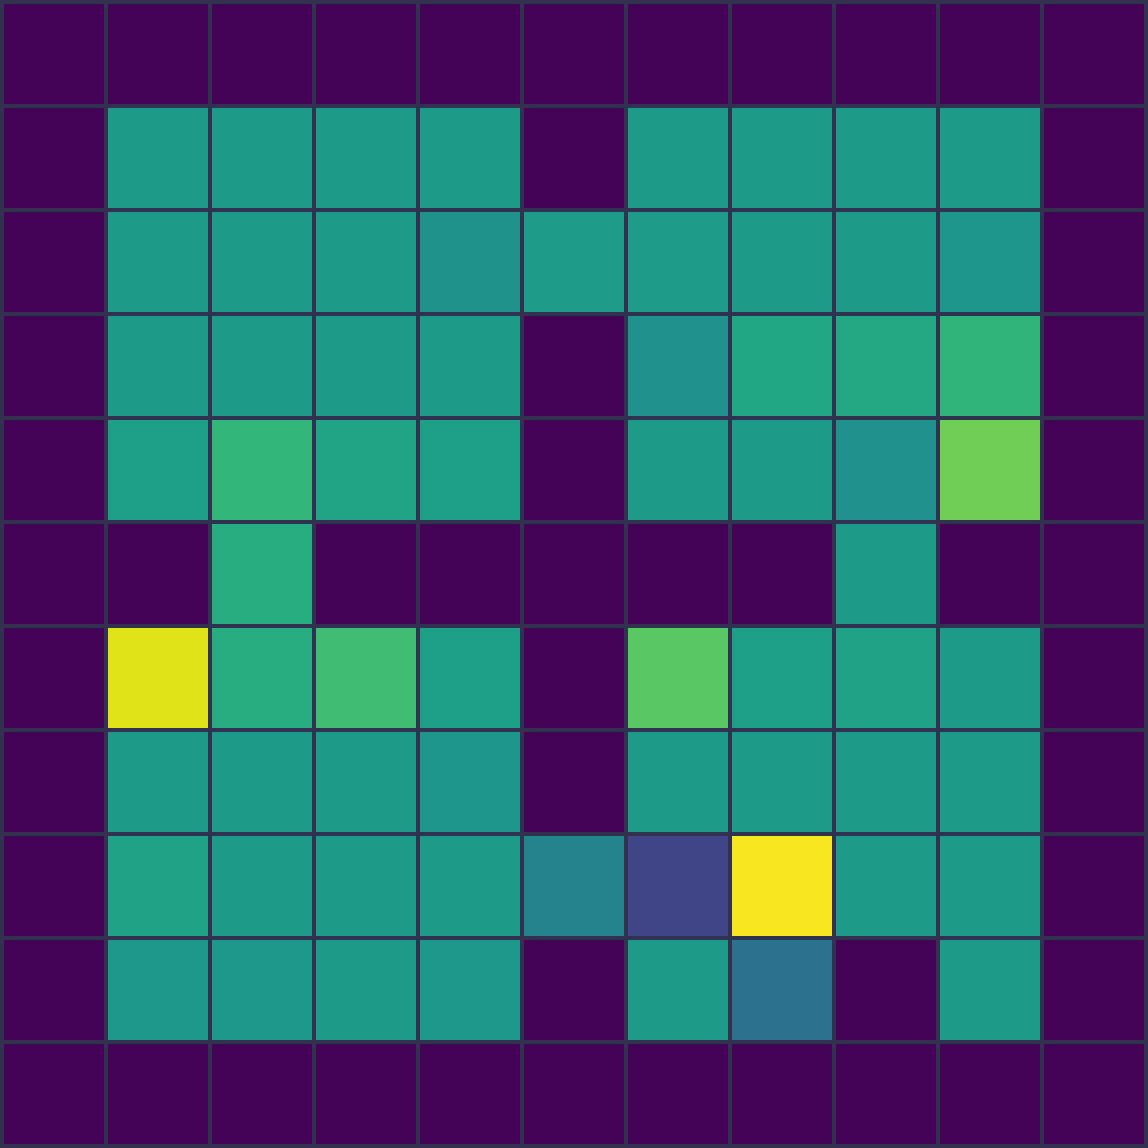
\includegraphics[width=0.09\textwidth]{image/chap04/prediction/18.png}
		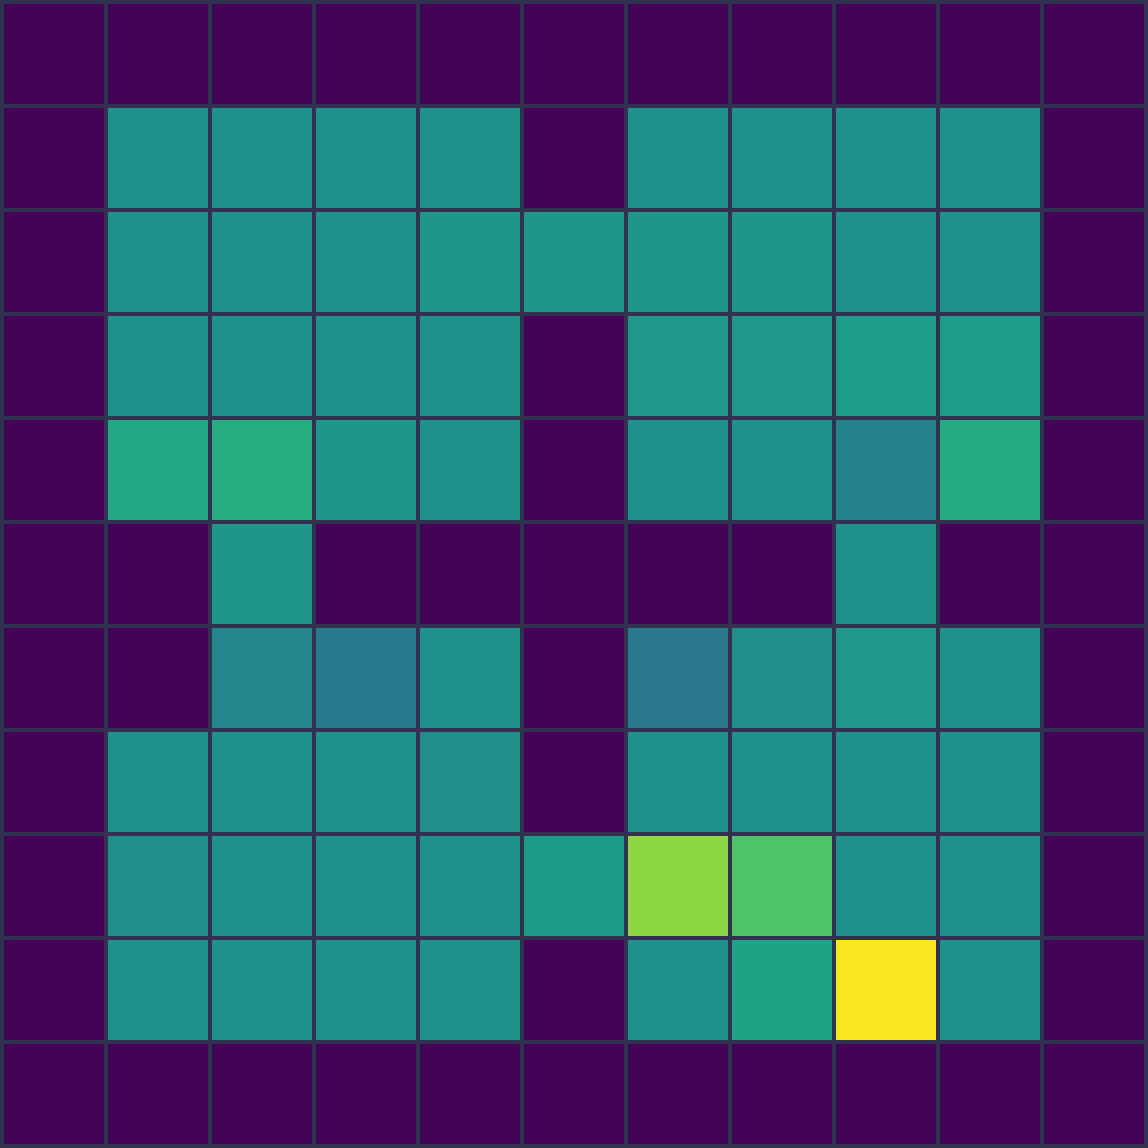
\includegraphics[width=0.09\textwidth]{image/chap04/prediction/19.png}
		\caption{预测向量}
		\label{fig:prediction}
	\end{figure}
}


\frame{
	\frametitle{实验结果}
	\begin{figure}[h!]
		\centering
		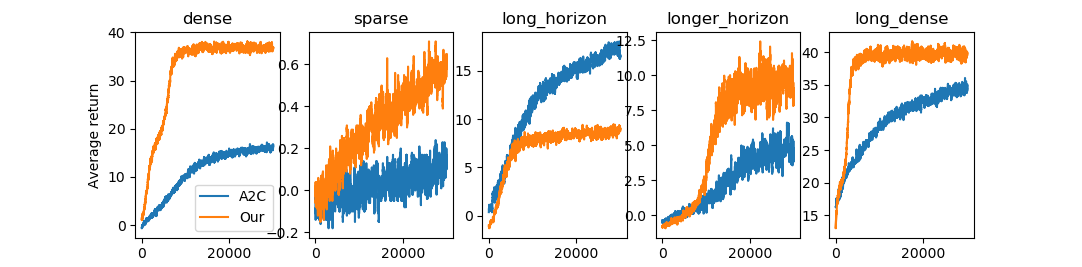
\includegraphics[width=1\textwidth]{image/chap04/tabular.png}
		\caption{网格世界的实验结果}
		\label{fig:tabular}
	\end{figure}
}

\endinput
